\section{Torque Sensor}
The purpose of the Torque Sensor is to measure the mechanical power which is given to the sensor in the form of rotational energy from the Roll. The sensor must be able to measure both torque $\tau$ and angular velocity $\omega$ as the power P is given by:
\begin{equation}
	P=\omega\cdot\tau
\end{equation}

As the Torque Sensor was chosen by the customer and as it is pre-mounted on the Roll Stand, the block will not be designed but will be analysed instead.

\subsection{Implementation}
The torque sensor picked by the customer is a DR-2212 Contactless Torque Sensor from Lorenz Messtechnik GmbH. The sensor is able to measure both the angular velocity and the torque applied to the input-shaft.

The torque sensor's input shaft is connected to the Roll and and the Generator's motor as seen on \vref{fig:Generator_Implementation}. The electrical outputs are given through a 12-pin connector as seen on figure \ref{fig:Torque_pins} below. The signals are transmitted from the sensor to the Control-box using a DE-9 connector.

\begin{figure}[H]
	\centering
	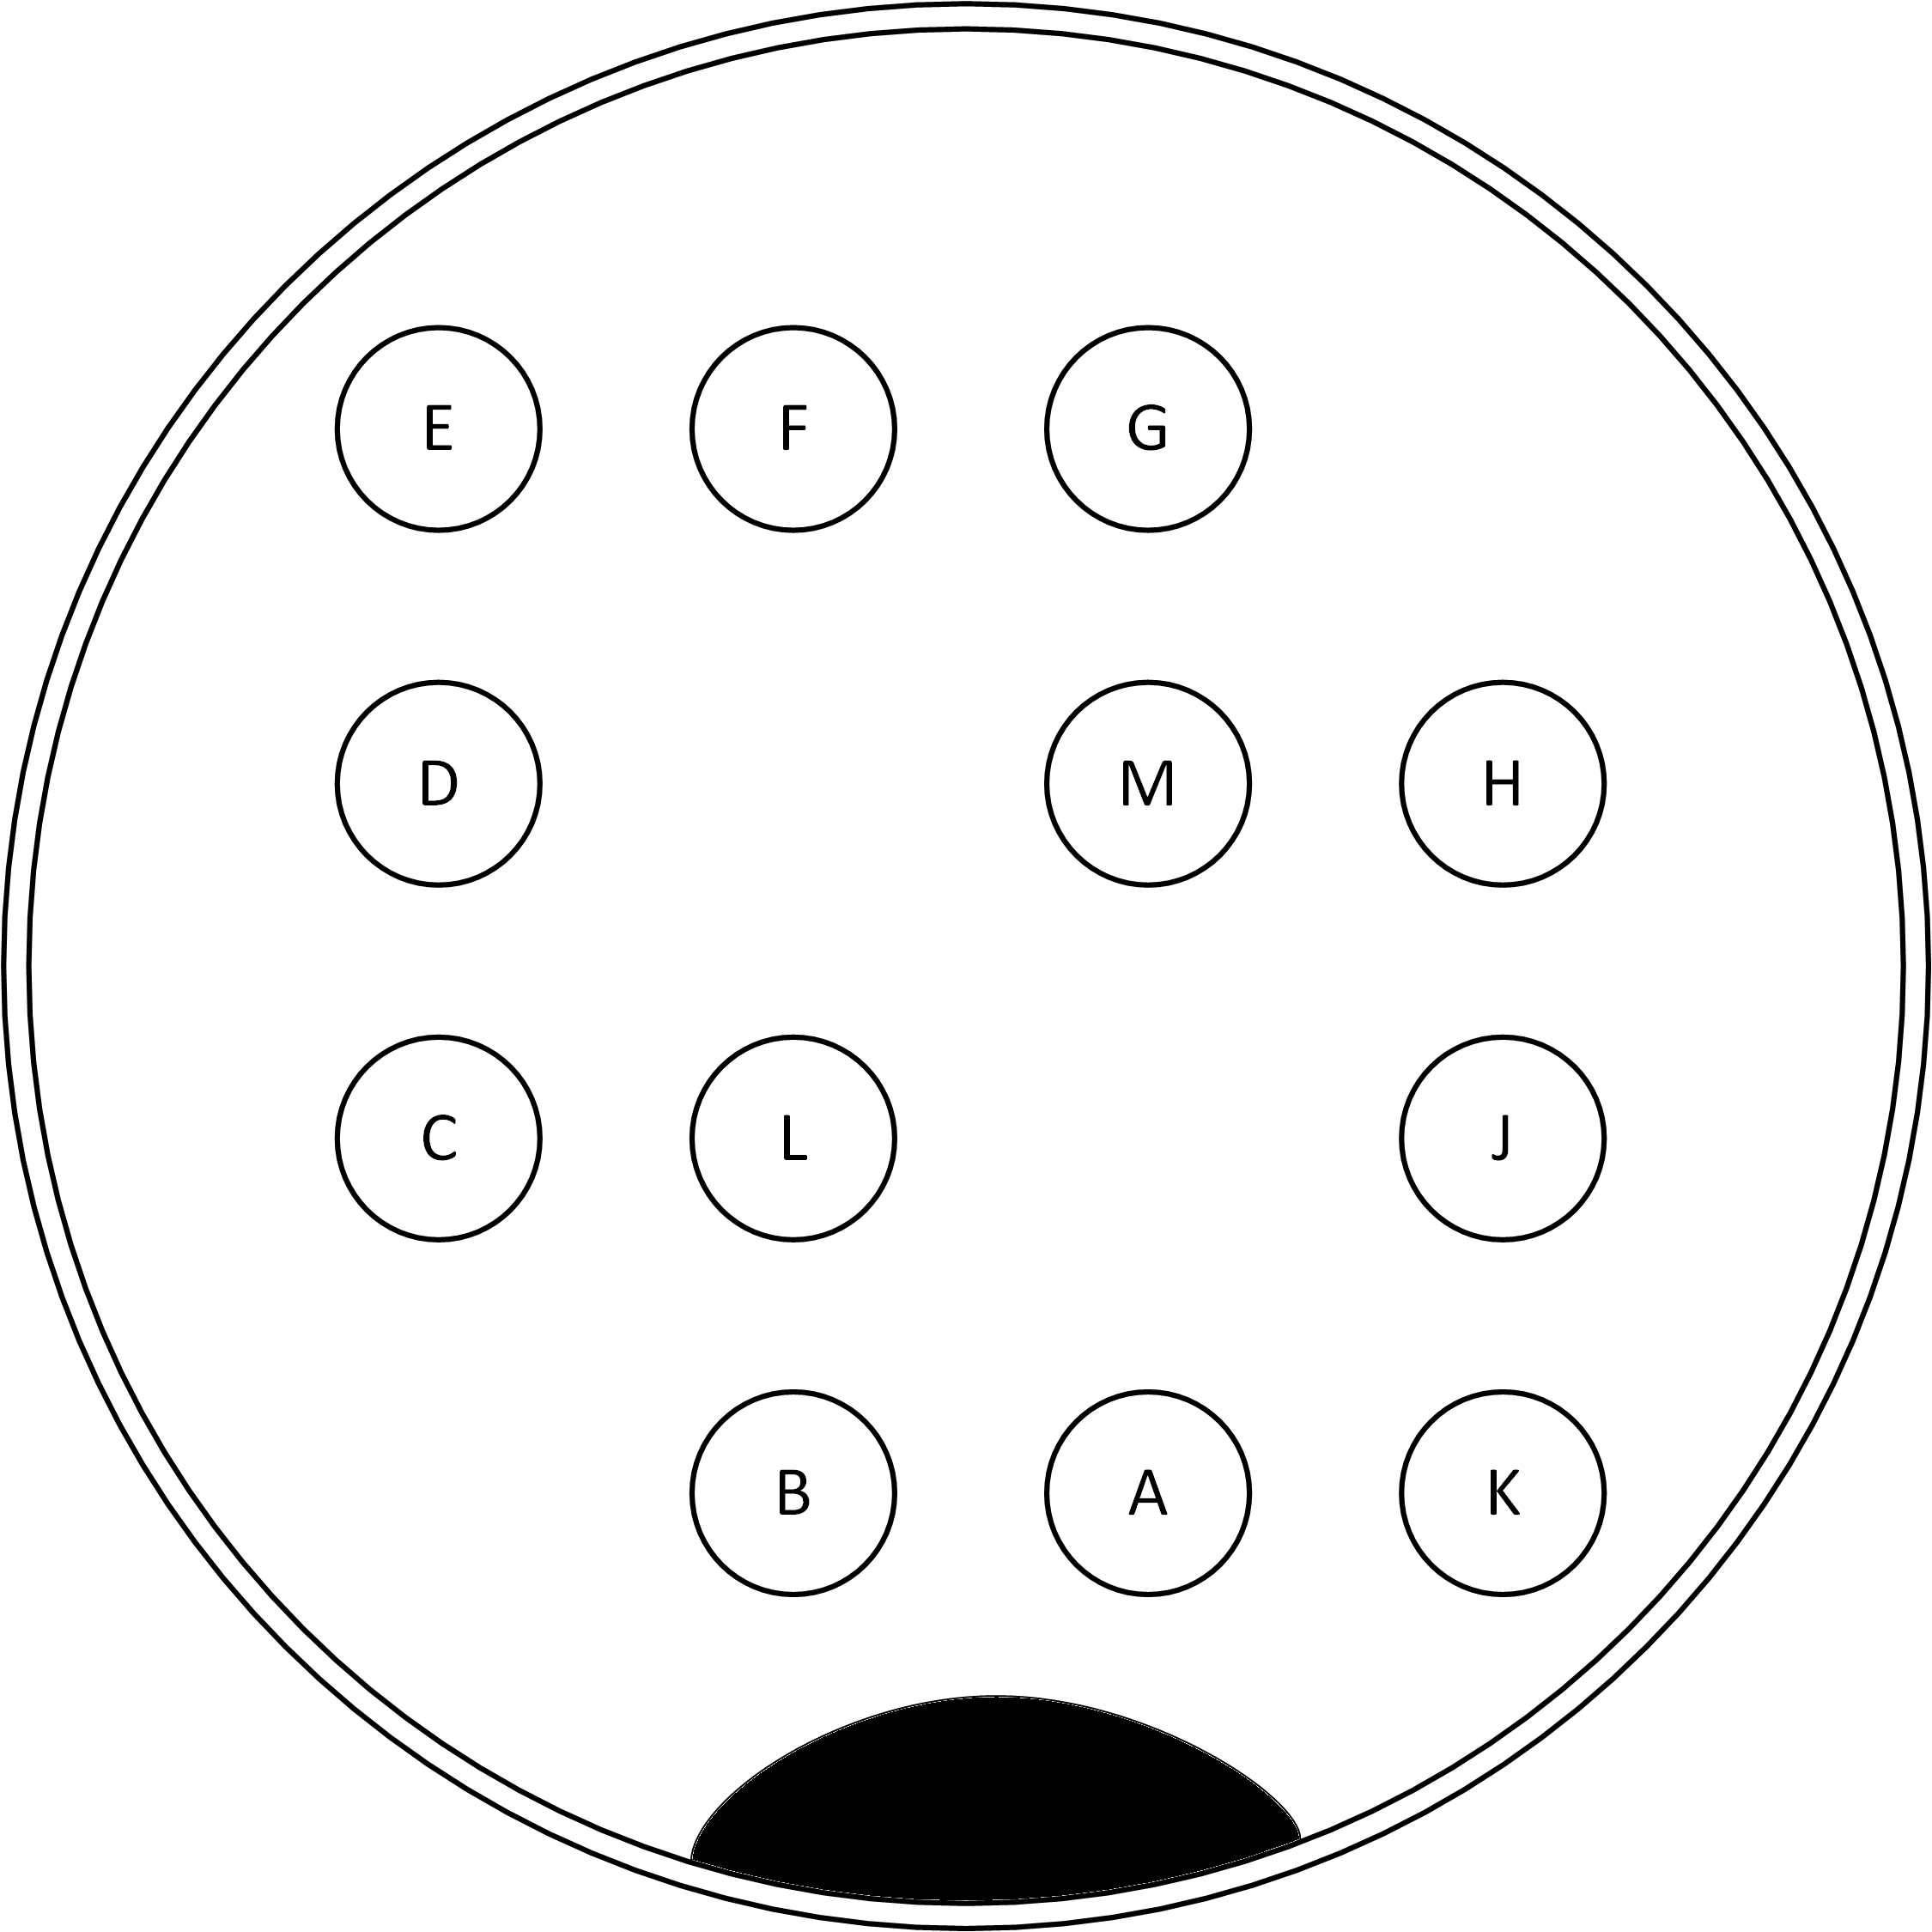
\includegraphics[width=0.4\linewidth]{Hardware/Pictures/Torque_Sensor_Pins}
	\caption{Torque Sensor pin configuration}
	\label{fig:Torque_pins}
\end{figure}

The Torque Sensor must be supplied with atleast 12 VDC, in order to power the internal µ-processor, and can therefore be connected directly to the Voltage Adaptor. The sensor can be supplied with higher DC-voltages (up to 28 VDC) but this would require an external power supply.

\subsection{Analysis}
The sensor specified to be able to measure torque levels ranging from $0$ to $5 Nm$ and angular velocity from $0$ to $30,000 rpm$. The sensor is able to measure these parameters irregardles of the input-shaft's rotational direction. Thus the mathematical limits of the sensor range from $-5 Nm$ to $+5 Nm$ and $-30,000 rpm$ to $+30,000 rpm$.

\textbf{Torque}\\
The Torque Sensor outputs the measured torque on Pin C (Signal+). The output-signal is a DC-voltage which is proportional to the measured torque - as long as the input value lies withing the specified range. An input outside this range would cause the sensor to reach saturation. The output-voltage range from $-5 V$ to $+5 V$ and the relationship between the input and output can therefore be expressed mathematically as:
\begin{equation}
	V_{sensor} = 
	\begin{cases}
		+5V				& \quad \text{if } \tau_{sensor} > +5 Nm\\
		\tau_{sensor}   & \quad \text{if } -5 Nm \leq V \leq +5 Nm\\
		-5V				& \quad \text{if } \tau_{sensor} < -5 Nm
	\end{cases}
\end{equation}

\textbf{Angular velocity}\\
The Torque Sensor outputs the measured angular velocity on Pin B (Angle B) and Pin G (Signal A) - however only the signal from Pin G is used for calculations. The output-signal is a square-waved signal with a DC-offset of 2.5 V and a peak-peak value of 5 V.

The output-signal changes level 360 times per axial revolution in the Torque Sensor. Thus the frequency of the signal is proportional to the angular velocity.

\subsection{Unity test}
Text